\documentclass{article}
\usepackage{amsmath,amssymb,amsthm}
\usepackage{fancyhdr}
\usepackage{enumerate}
\usepackage{graphicx}
\usepackage{caption}
\usepackage{float}

\pagestyle{fancy}
\fancyhf{}
\lhead{1st Homework - CSCE 312 503}
\rhead{Kevin Lei}
\renewcommand{\headrulewidth}{0.4pt}
\renewcommand{\arraystretch}{1.2}

\begin{document}

\section*{Question 1}
The way we solve this is using Amdahl's Law.
The formula for Amdahl's Law is: 
$$ S = \frac{1}{(1 - \alpha) + \frac{\alpha}{k}} $$
Where $S$ is the speedup, $\alpha$ is the fraction of the program that can be parallelized, and $k$ is the perfomance uplift.
\\ \\
In this situation, our $\alpha$ is 0.5, since half of the processing time is spent on floating-point instructions.
Since the enhancement has allowed the machine to run floating-point instructions five times faster, our $k$ is 5.
Putting all this into our equation, we get
\begin{align*}
S &= \frac{1}{(1 - 0.5) + \frac{0.5}{5}} \\
&= \frac{1}{0.5 + 0.1} \\
&= \frac{1}{0.6} \\
&\approx 1.67 \; .
\end{align*}
Thus, our overall speedup is 1.67.

\section*{Question 2}

\subsection*{a)}
Here we need to figure out which one of the optimizations has the greater effect on the performance.
If we only make the divide operation 3 times faster, we have an overall speedup of
\begin{align*}
    S &= \frac{1}{(1 - 0.2) + \frac{0.2}{3}} \\
    &= \frac{1}{0.8 + \frac{1}{15}} \\
    &\approx 1.15 \; \text{times.}
\end{align*}
If we only make the multiple operation 8 times faster, we have an overall speedup of
\begin{align*}
    S &= \frac{1}{(1 - 0.6) + \frac{0.6}{8}} \\
    &= \frac{1}{0.4 + \frac{3}{40}} \\
    &\approx 2.11 \; \text{times.}
\end{align*}
Therefore, we cannot meet management's goal of achieving a 5 times performance uplift by only making either the divide or multiply operation faster, 
as the maximum speedup we can achieve is 2.11 times with only the multiply operation being 8 times faster.

\subsection*{b)}
Amdahl's law works by diving the old time by the new time to get the speedup, which makes intuitive sense.
If the old time is 1, the new time can be found by removing the parts that are sped up and adding the speed adjusted parts back in.
Thus we can generalize Amdahl's law to multiple speedups:
$$ S = \frac{1}{(1 - \alpha - \beta) + \frac{\alpha}{k_1} + \frac{\beta}{k_2}} $$
Where $\alpha$ and $\beta$ are the fractions of the program that can be parallelized, and $k_1$ and $k_2$ are their respective perfomance uplifts.
Now we can use this to find the overall speedup if we make both improvements.
\begin{align*}
    S &= \frac{1}{(1 - 0.2 - 0.6) + \frac{0.2}{3} + \frac{0.6}{8}} \\
    &= \frac{1}{0.2 + \frac{1}{15} + \frac{3}{40}} \\
    &\approx 2.93 \; .
\end{align*}
Now, our speedup relative to the old machine is 2.93 times.

\newpage
\section*{Textbook Problems:}
\textit{Digital Design, 2nd Ed, by Frank Vahid, Wiley publication, 2010}

\subsection*{1.8}
Binary to decimal:
\begin{enumerate}[(a)]
    \item $100 = 2^2 = 4$
    \item $1011 = 2^3 + 2^1 + 2^0 = 8 + 2 + 1 = 11$
    \item $0000000000001 = 1$
    \item $111111 = 2^0 + 2^1 + 2^2 + 2^3 + 2^4 + 2^5 = 1 + 2 + 4 + 8 + 16 + 32 = 63$
    \item $101010 = 2^1 + 2^3 + 2^5 = 2 + 8 + 32 = 42$
\end{enumerate}

\subsection*{1.15}
Decimal to binary using divide by 2:
\begin{enumerate}[(a)]
    \item 
    $19 \div 2 = 9 \text{ remainder } 1$ \\
    $9 \div 2 = 4 \text{ remainder } 1$ \\
    $4 \div 2 = 2 \text{ remainder } 0$ \\
    $2 \div 2 = 1 \text{ remainder } 0$ \\
    $1 \div 2 = 0 \text{ remainder } 1$ \\
    $19 = 10011$
    \item 
    $30 \div 2 = 15 \text{ remainder } 0$ \\
    $15 \div 2 = 7 \text{ remainder } 1$ \\
    $7 \div 2 = 3 \text{ remainder } 1$ \\
    $3 \div 2 = 1 \text{ remainder } 1$ \\
    $1 \div 2 = 0 \text{ remainder } 1$ \\
    $30 = 11110$
    \item 
    $64 \div 2 = 32 \text{ remainder } 0$ \\
    $32 \div 2 = 16 \text{ remainder } 0$ \\
    $16 \div 2 = 8 \text{ remainder } 0$ \\
    $8 \div 2 = 4 \text{ remainder } 0$ \\
    $4 \div 2 = 2 \text{ remainder } 0$ \\
    $2 \div 2 = 1 \text{ remainder } 0$ \\
    $1 \div 2 = 0 \text{ remainder } 1$ \\
    $64 = 1000000$
    \newpage
    \item 
    $128 \div 2 = 64 \text{ remainder } 0$ \\
    $64 \div 2 = 32 \text{ remainder } 0$ \\
    $32 \div 2 = 16 \text{ remainder } 0$ \\
    $16 \div 2 = 8 \text{ remainder } 0$ \\
    $8 \div 2 = 4 \text{ remainder } 0$ \\
    $4 \div 2 = 2 \text{ remainder } 0$ \\
    $2 \div 2 = 1 \text{ remainder } 0$ \\
    $1 \div 2 = 0 \text{ remainder } 1$ \\
    $128 = 10000000$
\end{enumerate}

\subsection*{1.18}
Binary to hexadecimal:
\begin{enumerate}[(a)]
    \item $11110000 = F0$
    \item $11111111 = FF$
    \item $01011010 = 5A$
    \item $1001101101101 = 136D$
\end{enumerate}

\subsection*{1.22}
Hexadecimal to binary:
\begin{enumerate}[(a)]
    \item $4F5E = 0100111101011110$
    \item $3FAD = 0011111110101101$
    \item $3E2A = 0011111000101010$
    \item $DEED = 1101111011101101$
\end{enumerate}

\subsection*{1.32}
We want to minimize the amount of custom ditital circuitry while maintaining at least 40 transactions per second.
With only microprocessors, one transaction consisting of subtasks A, B, and C takes 0.05 s + 0.02 s + 0.02 s = 0.09 s.
Thus, the maximum number of transactions per second is $\frac{1}{0.09} \approx 11.11$ transactions per second.
Switching out the microprocessor for custom digital circuitry on part A gives us the largest upfront improvement from 50 ms to 1 ms.
Now the maximum number of transactions per second is $\frac{1}{0.001 + 0.02 + 0.02} \approx 24.39$ transactions per second.
Replacing the microprocessor with custom digital circuitry on part C gives us the next largest improvement from 20 ms to 1 ms.
Now the maximum number of transactions per second is $\frac{1}{0.001 + 0.02 + 0.001} \approx 45.45$ transactions per second.
Thus, the best way to achieve the goal of at least 40 transactions per second is to replace the microprocessor with custom digital circuitry on parts A and C.

\subsection*{2.12}
Evaluate $F = (a \; AND \; b) \; OR \; c \; OR \; d$ for the following values of $a$, $b$, $c$, and $d$:
\begin{enumerate}
    \item $a = 1$, $b = 1$, $c = 1$, $d = 0$ \\
    $ F = 1*1 + 1 + 0 = 1 $
    \item $a = 0$, $b = 1$, $c = 1$, $d = 0$ \\
    $ F = 0*1 + 1 + 0 = 1 $
    \item $a = 1$, $b = 1$, $c = 0$, $d = 0$ \\
    $ F = 1*1 + 0 + 0 = 1 $
    \item $a = 1$, $b = 0$, $c = 0$, $d = 0$ \\
    $ F = 1*0 + 0 + 0 = 0 $
\end{enumerate}

\subsection*{2.18}
Convert to gate level circuits:
\begin{enumerate}[(a)]
    \item $F = a'b' + b'c$
    \begin{figure}[h]
        \centering
        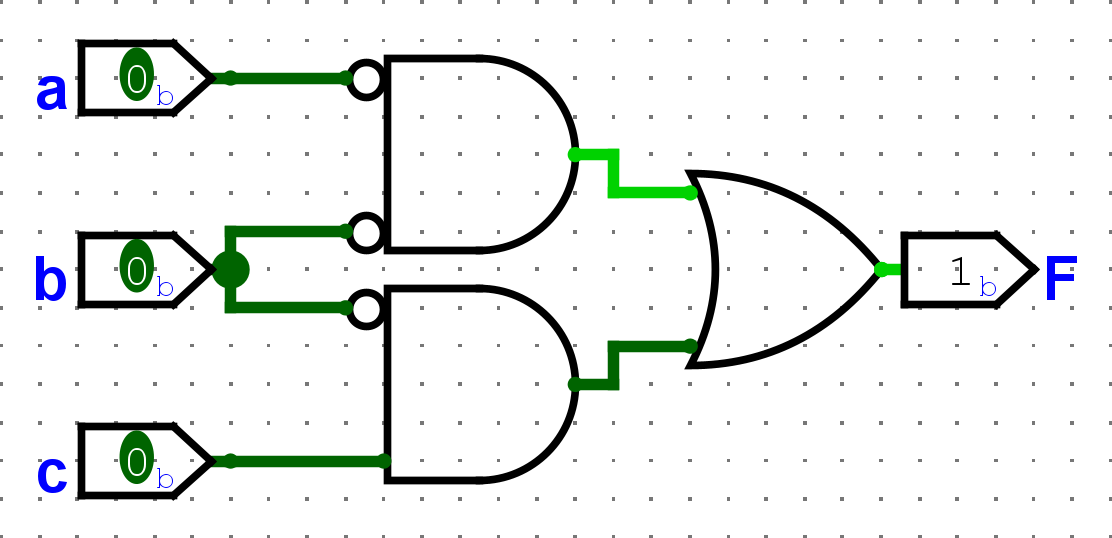
\includegraphics[width=0.5\textwidth]{./images/2_18_a.png}
    \end{figure}
    \item $F = ab + bc + cd + de$
    \begin{figure}[h]
        \centering
        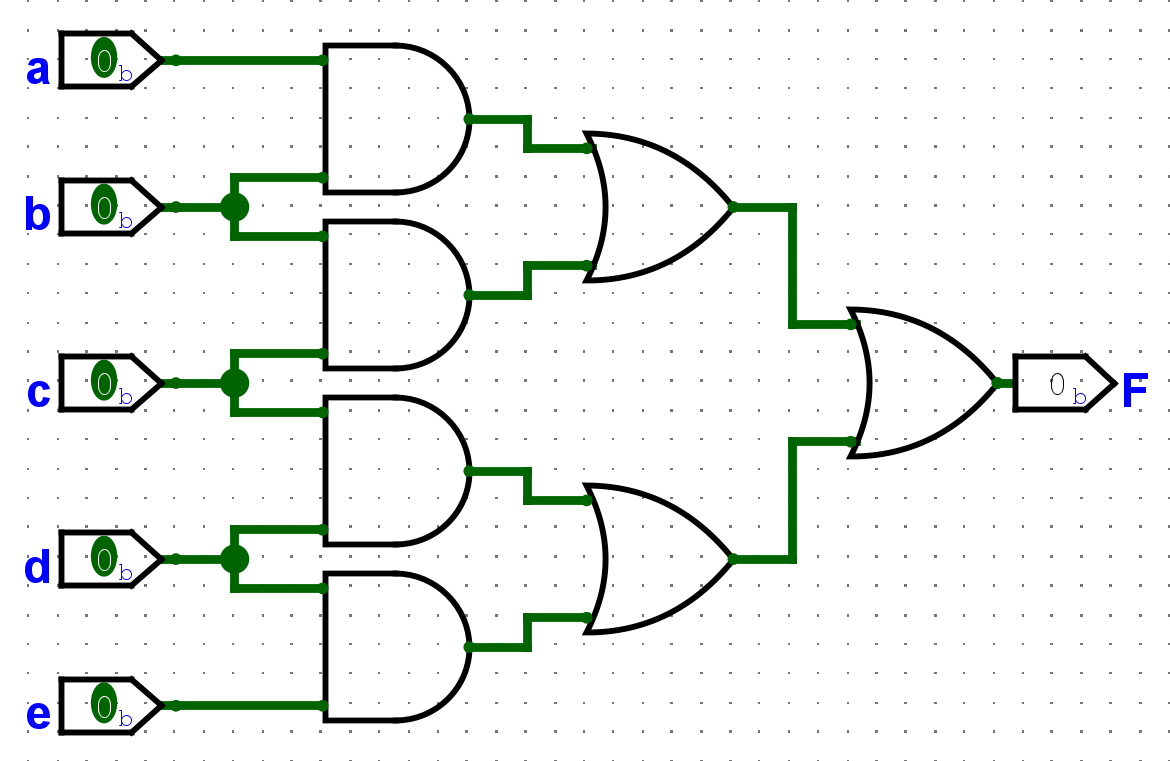
\includegraphics[width=0.5\textwidth]{./images/2_18_b.png}
    \end{figure}
    \newpage
    \item $F = ((ab)' + (c)) + (d + ef)'$
    \begin{figure}[h]
        \centering
        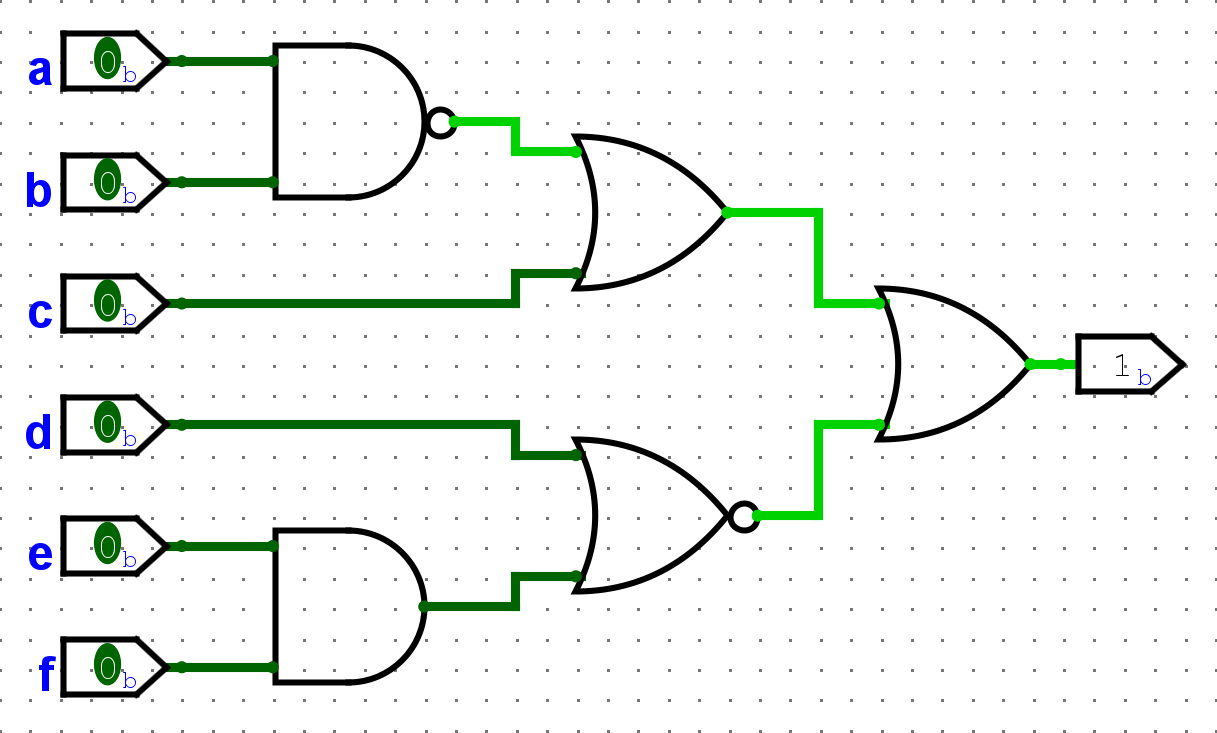
\includegraphics[width=0.5\textwidth]{./images/2_18_c.png}
    \end{figure}
\end{enumerate}

\subsection*{2.24}
For the function $F = a'd' + a'c + b'cd' + cd$:
\begin{enumerate}[(a)]
    \item List all the variables. \\
    We have variables $a$, $b$, $c$, and $d$.
    \item List all the literals. \\
    We have literals $a$, $a'$, $b$, $b'$, $c$, $c'$, $d$, and $d'$.
    \item List all the product terms.
    The product terms are $a'd'$, $a'c$, $b'cd'$, and $cd$.
\end{enumerate}

\subsection*{2.28}
Convert to sum of products form: $F = a'b(c + d') + a(b' + c) + a(b + d)c$
\begin{align*}
    F &= a'b(c + d') + a(b' + c) + a(b + d)c \\
    &= a'bc + a'bd' + ab' + ac + abc + acd
\end{align*}

\subsection*{2.33}
The circuit converted to a boolean expression is: \\
$ G = ab' + b + a'c $

\subsection*{2.39}
The truth table of $F$ converted to a boolean expression is: \\
$ F = a'b'c' + a'bc' + ab'c' + ab'c + abc' $

\newpage
\subsection*{2.52}
Determine if $F$ and $G$ are equivalent using (a) algebraic manipulation and (b) truth tables: \\
$$ F = ab + cd $$
$$ G = (1((ab)'(cd)')')' $$

\noindent (a) Algebraic manipulation \\
\begin{align*}
    G &= (1((ab)'(cd)')')' \\
    &= 0 + ((ab)'(cd)')' \\
    &= ab + cd \\
    &= F
\end{align*}

\noindent (b) Comparing truth tables \\
\begin{minipage}{.4\textwidth}
\centering
\begin{tabular}{c c c c|c}
    a & b & c & d & F \\
    \hline
    0 & 0 & 0 & 0 & 0 \\
    0 & 0 & 0 & 1 & 0 \\
    0 & 0 & 1 & 0 & 0 \\
    0 & 0 & 1 & 1 & 1 \\
    0 & 1 & 0 & 0 & 0 \\
    0 & 1 & 0 & 1 & 1 \\
    0 & 1 & 1 & 0 & 0 \\
    0 & 1 & 1 & 1 & 1 \\
    1 & 0 & 0 & 0 & 0 \\
    1 & 0 & 0 & 1 & 0 \\
    1 & 0 & 1 & 0 & 0 \\
    1 & 0 & 1 & 1 & 1 \\
    1 & 1 & 0 & 0 & 1 \\
    1 & 1 & 0 & 1 & 1 \\
    1 & 1 & 1 & 0 & 1 \\
    1 & 1 & 1 & 1 & 1 \\
\end{tabular}
\captionof{table}{Truth table for $F$}
\end{minipage}
\begin{minipage}{.4\textwidth}
\centering
\begin{tabular}{c c c c|c}
    a & b & c & d & G \\
    \hline
    0 & 0 & 0 & 0 & 0 \\
    0 & 0 & 0 & 1 & 0 \\
    0 & 0 & 1 & 0 & 0 \\
    0 & 0 & 1 & 1 & 1 \\
    0 & 1 & 0 & 0 & 0 \\
    0 & 1 & 0 & 1 & 1 \\
    0 & 1 & 1 & 0 & 0 \\
    0 & 1 & 1 & 1 & 1 \\
    1 & 0 & 0 & 0 & 0 \\
    1 & 0 & 0 & 1 & 0 \\
    1 & 0 & 1 & 0 & 0 \\
    1 & 0 & 1 & 1 & 1 \\
    1 & 1 & 0 & 0 & 1 \\
    1 & 1 & 0 & 1 & 1 \\
    1 & 1 & 1 & 0 & 1 \\
    1 & 1 & 1 & 1 & 1 \\
\end{tabular}
\captionof{table}{Truth table for $G$}
\end{minipage} \\
\noindent We can see that the truth tables for $F$ and $G$ are the same, so $F$ and $G$ are equivalent.

\newpage
\subsection*{2.58}
$P = N_3'(N_2' N_1 + N_0) + N_3 N_0 (N_2 \oplus N_1)$
\begin{figure}[H]
    \centering
    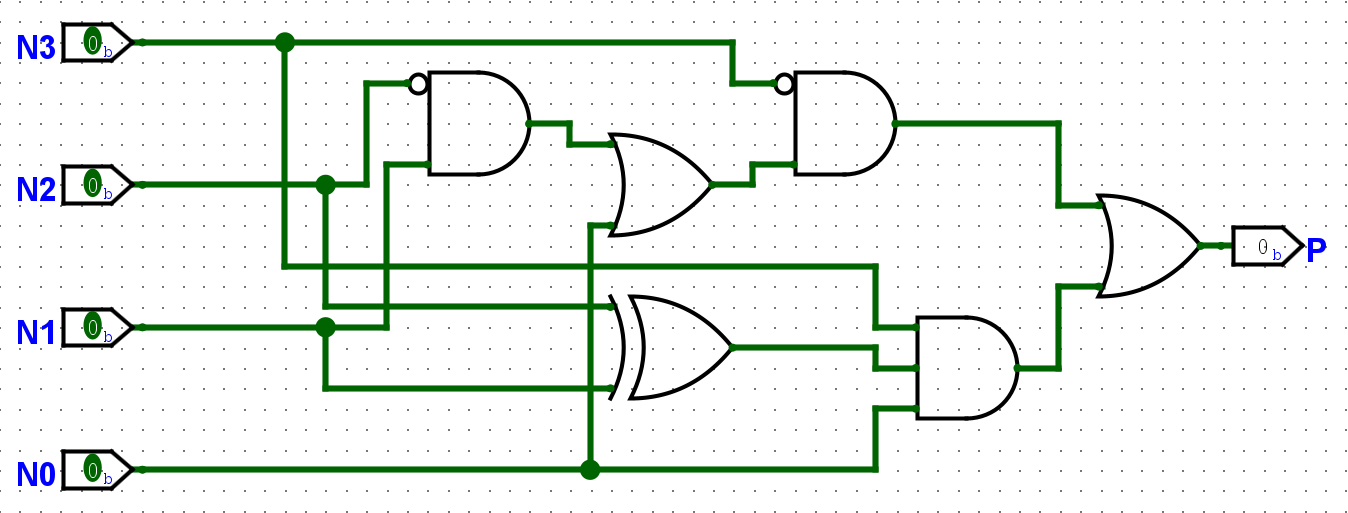
\includegraphics[width=0.75\textwidth]{./images/2_58.png}
\end{figure}

\subsection*{2.66}
\begin{figure}[H]
    \centering
    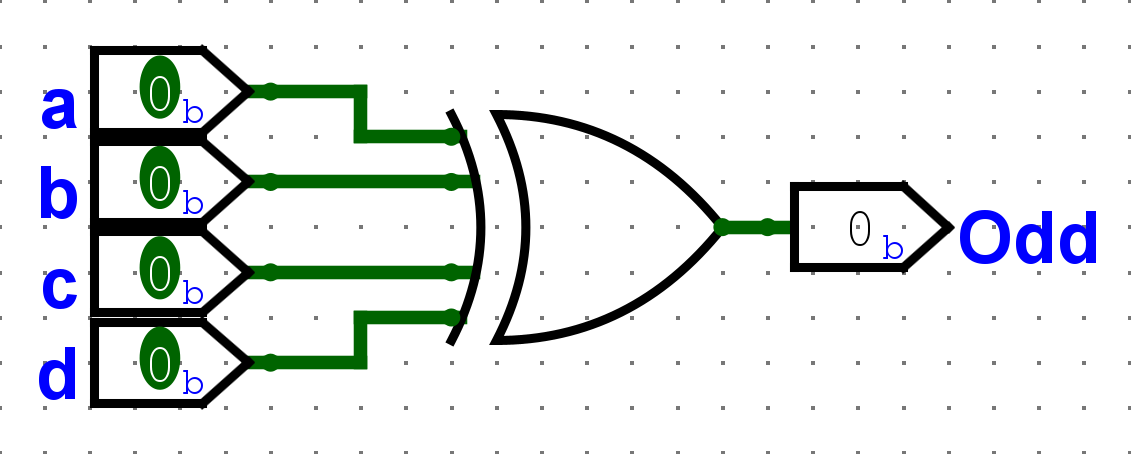
\includegraphics[width=0.4\textwidth]{./images/2_66.png}
\end{figure}

\subsection*{2.70}
\begin{figure}[H]
    \centering
    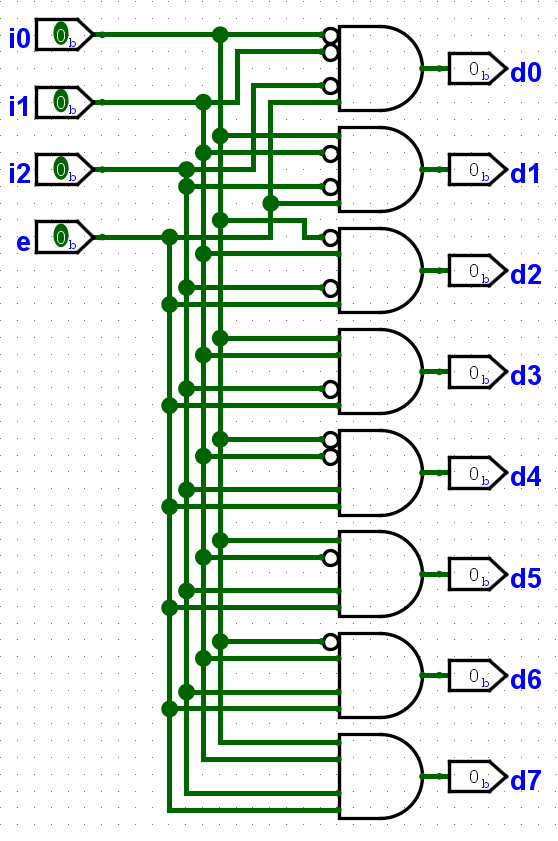
\includegraphics[width=0.5\textwidth]{./images/2_70.png}
\end{figure}

\subsection*{2.71}
\begin{figure}[H]
    \centering
    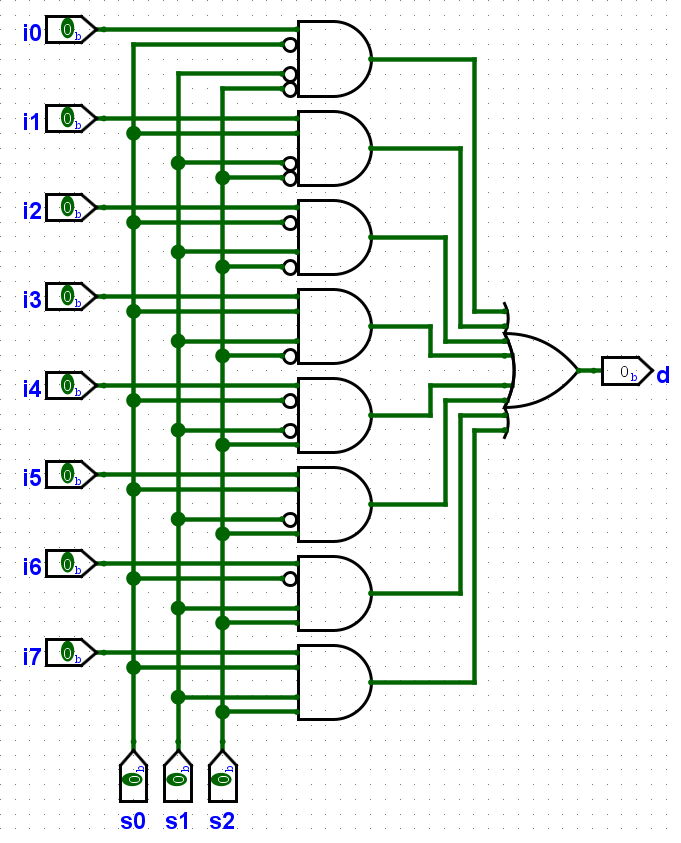
\includegraphics[width=0.66\textwidth]{./images/2_71.png}
\end{figure}

\subsection*{2.75}
\begin{figure}[H]
    \centering
    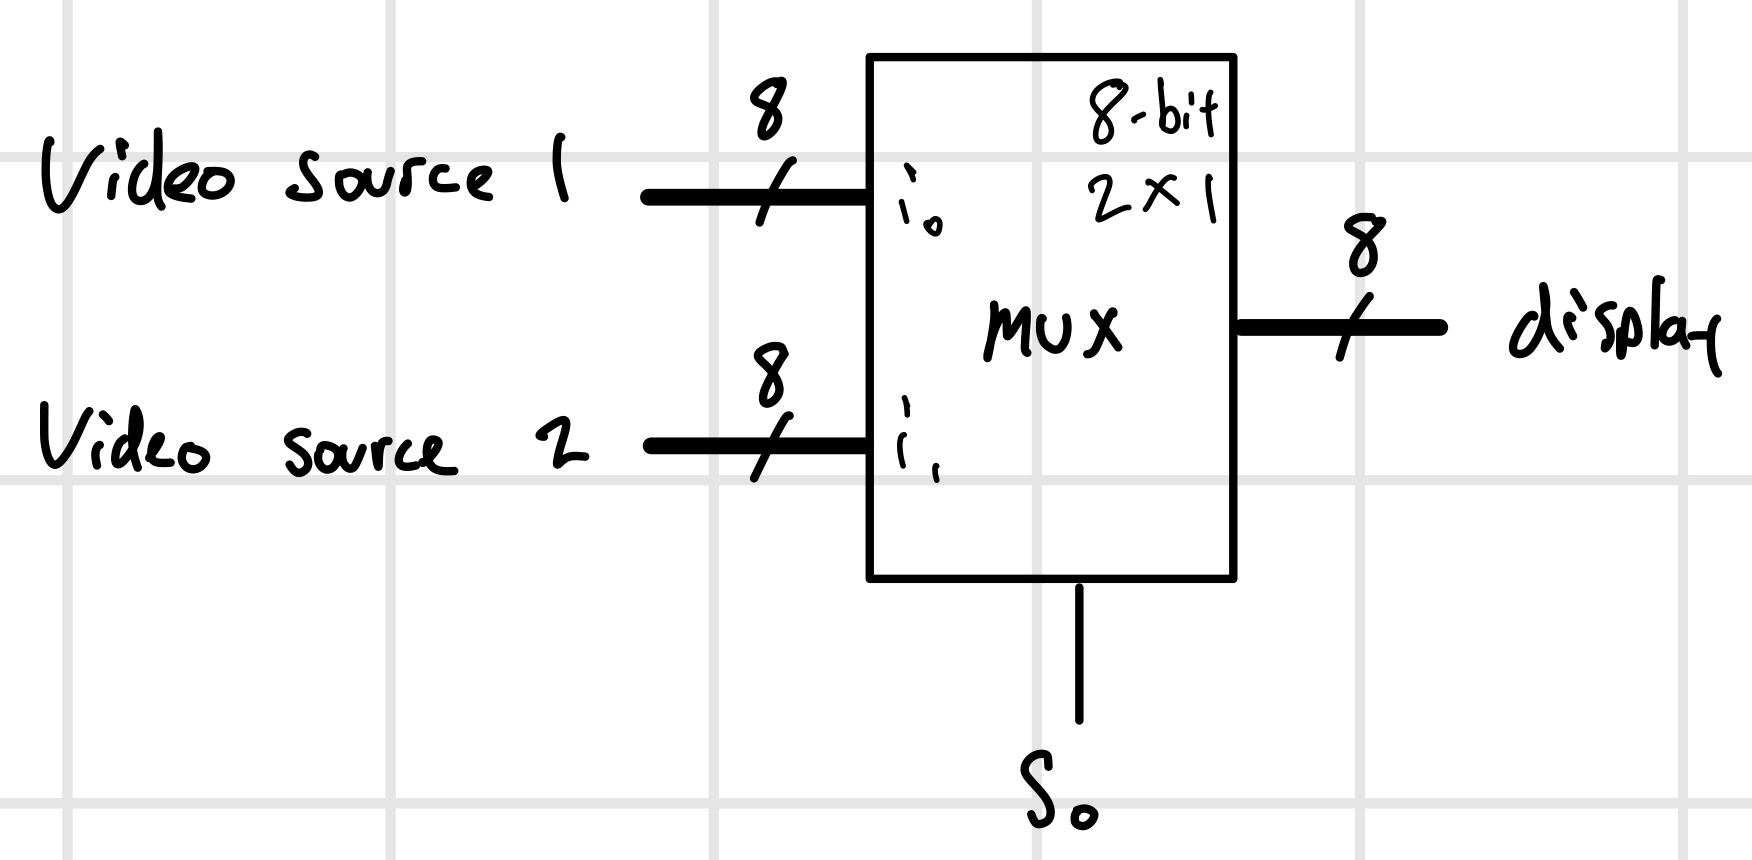
\includegraphics[width=0.69\textwidth]{./images/2_75.jpg}
\end{figure}

\newpage
\subsection*{3.2}
Clock period of frequencies:
\begin{enumerate}[(a)]
    \item 32.768 kHz has a period of $\frac{1}{32.768 \times 10^3} \approx 3.052 \times 10^{-5}$ s
    \item 100 MHz has a period of $\frac{1}{100 \times 10^6} = 1 \times 10^{-8}$ s
    \item 1.5 GHz has a period of $\frac{1}{1.5 \times 10^9} = 6.67 \times 10^{-10}$ s
    \item 2.4 GHz has a period of $\frac{1}{2.4 \times 10^9} = 4.17 \times 10^{-10}$ s
\end{enumerate}

\subsection*{3.4}
Frequency of clock periods:
\begin{enumerate}[(a)]
    \item 500 ms has a frequency of $\frac{1}{500 \times 10^{-3}} = 2$ Hz
    \item 400 ns has a frequency of $\frac{1}{400 \times 10^{-9}} = 2.5 \times 10^6$ Hz
    \item 4 ns has a frequency of $\frac{1}{4 \times 10^{-9}} = 2.5 \times 10^8$ Hz
    \item 20 ps has a frequency of $\frac{1}{20 \times 10^{-12}} = 5 \times 10^{11}$ Hz
\end{enumerate}

\subsection*{3.10}
\begin{figure}[H]
    \centering
    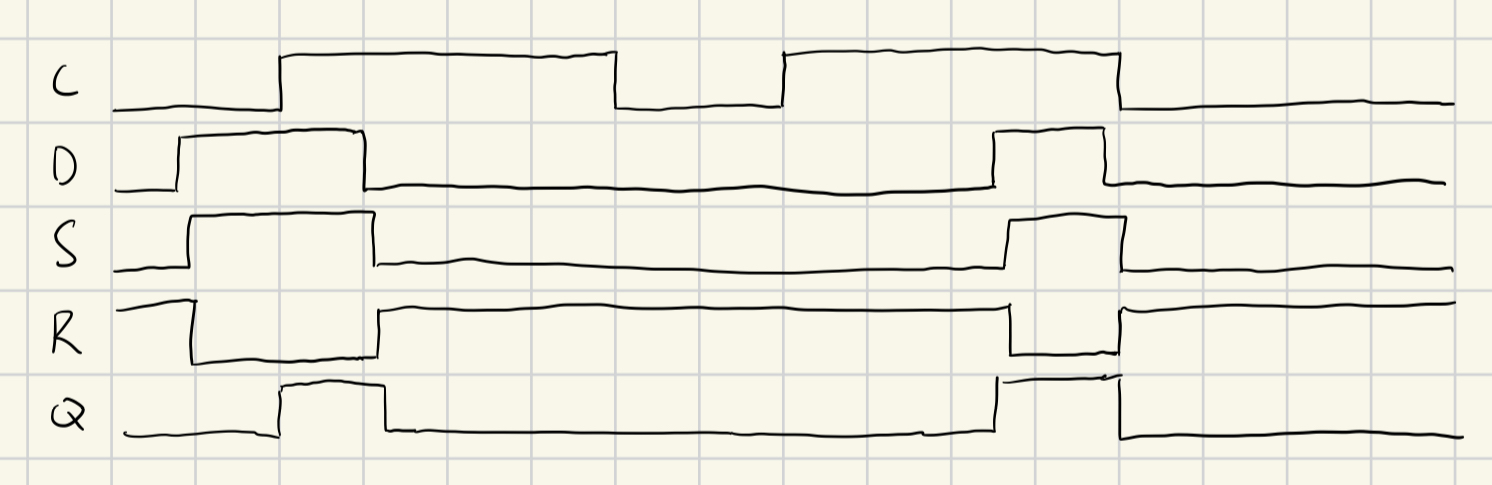
\includegraphics[width=\textwidth]{./images/3_10.jpg}
\end{figure}

\subsection*{3.12}
\begin{figure}[H]
    \centering
    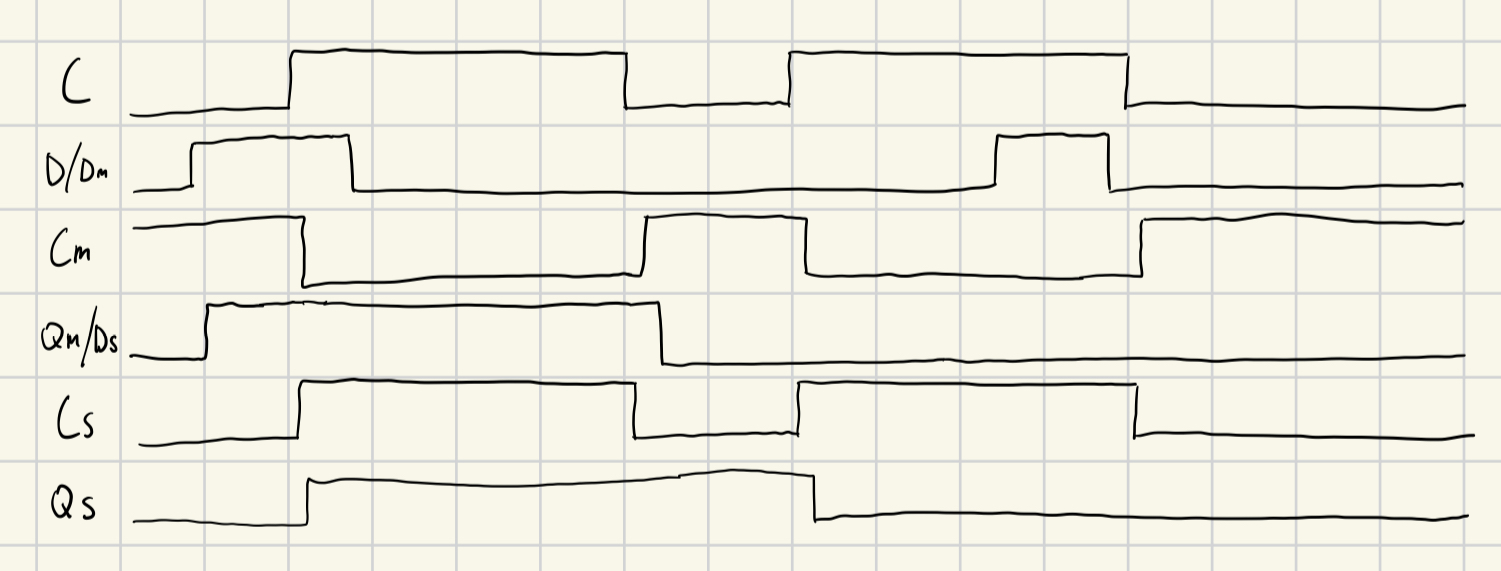
\includegraphics[width=\textwidth]{./images/3_12.jpg}
\end{figure}

\subsection*{3.21}
\begin{figure}[H]
    \centering
    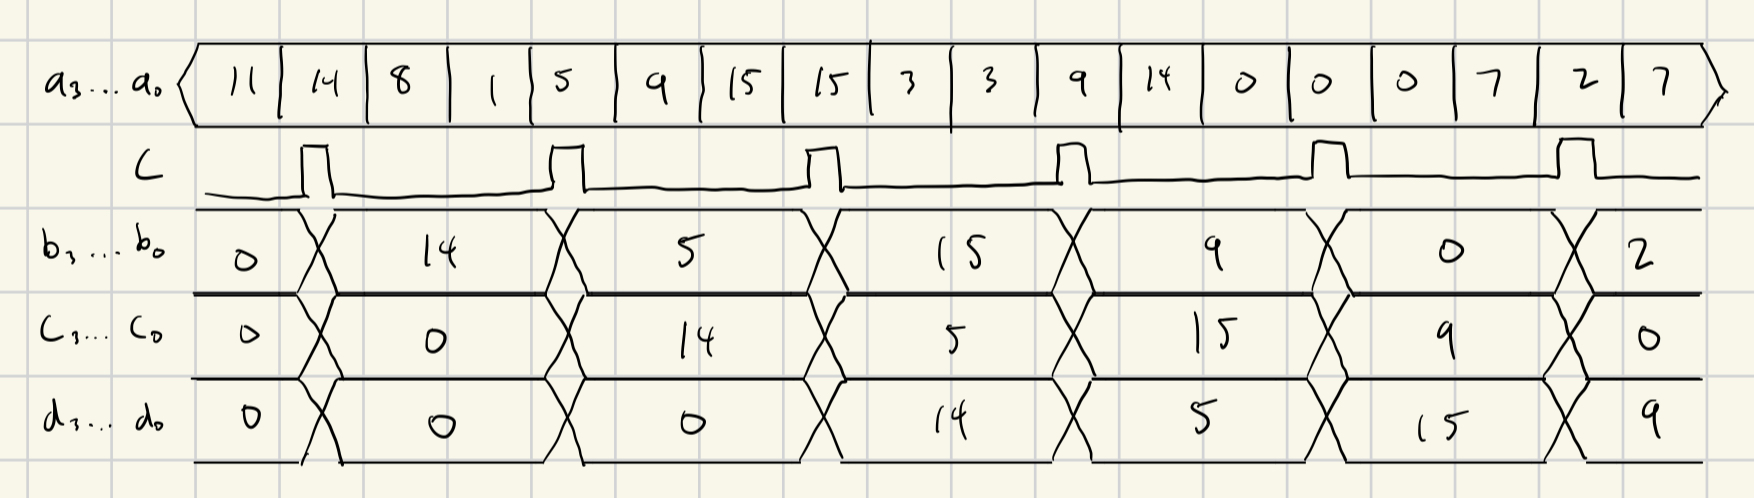
\includegraphics[width=\textwidth]{./images/3_21.jpg}
\end{figure}

\subsection*{3.30}
\begin{figure}[H]
    \centering
    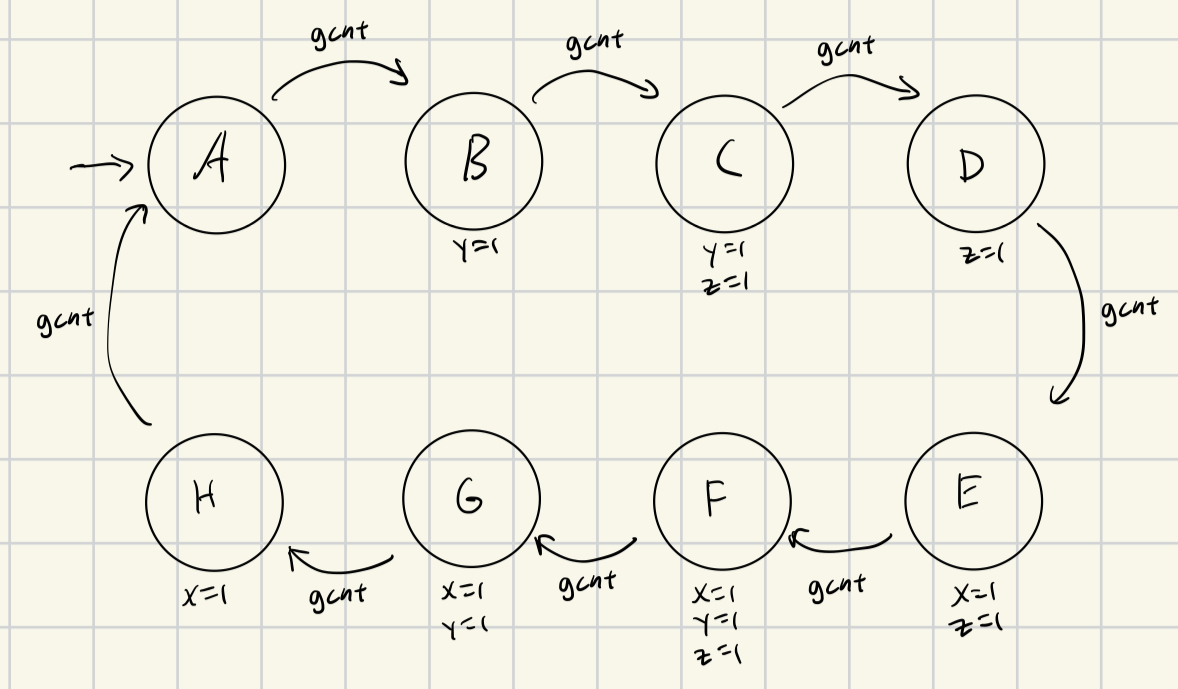
\includegraphics[width=\textwidth]{./images/3_30.jpg}
\end{figure}

\subsection*{3.40}
\begin{figure}[H]
    \centering
    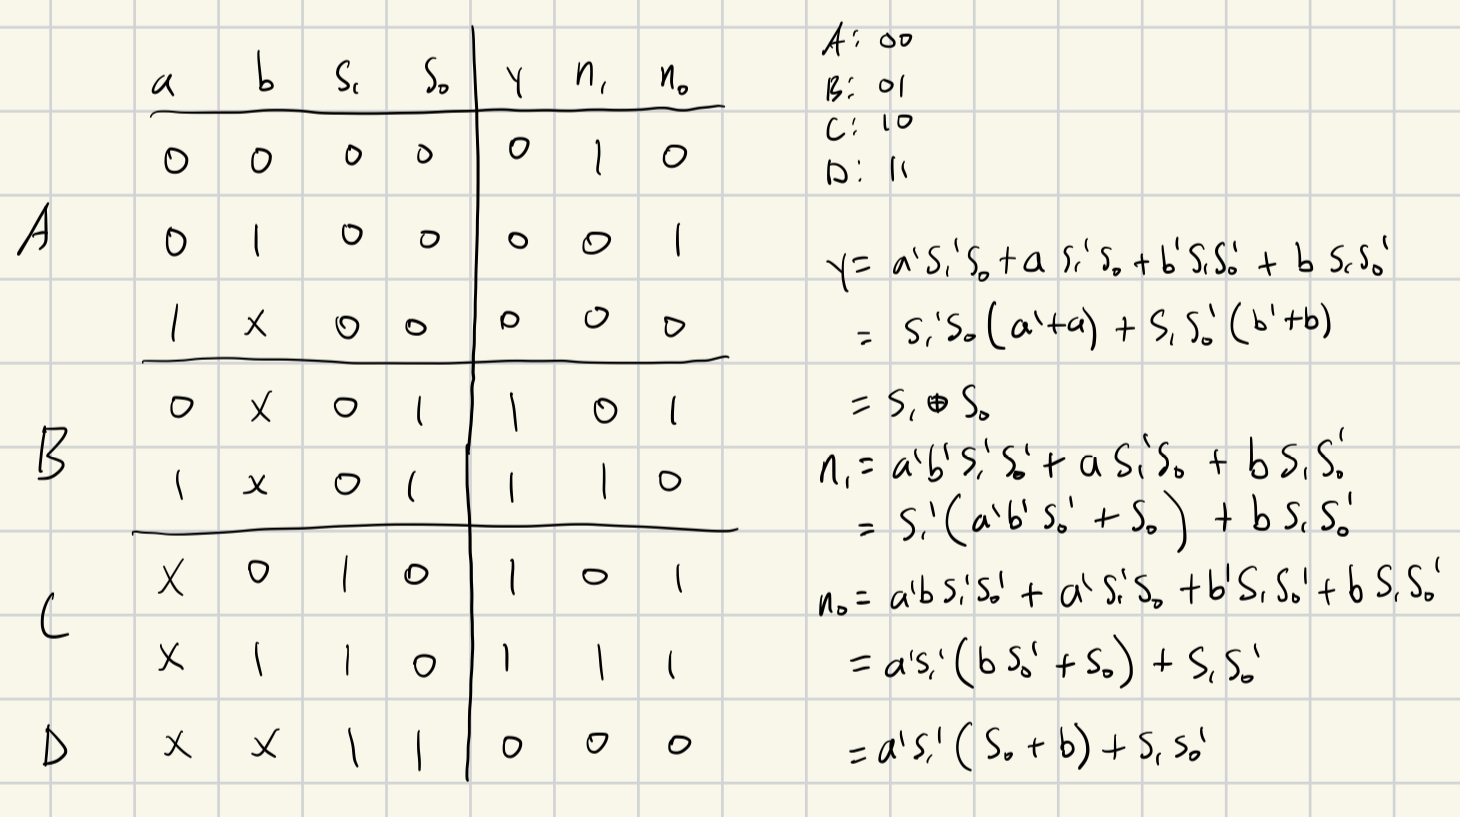
\includegraphics[width=\textwidth]{./images/3_40.jpg}
    \caption*{Truth table and boolean expressions for the finite state machine.}
\end{figure}

\begin{figure}[H]
    \centering
    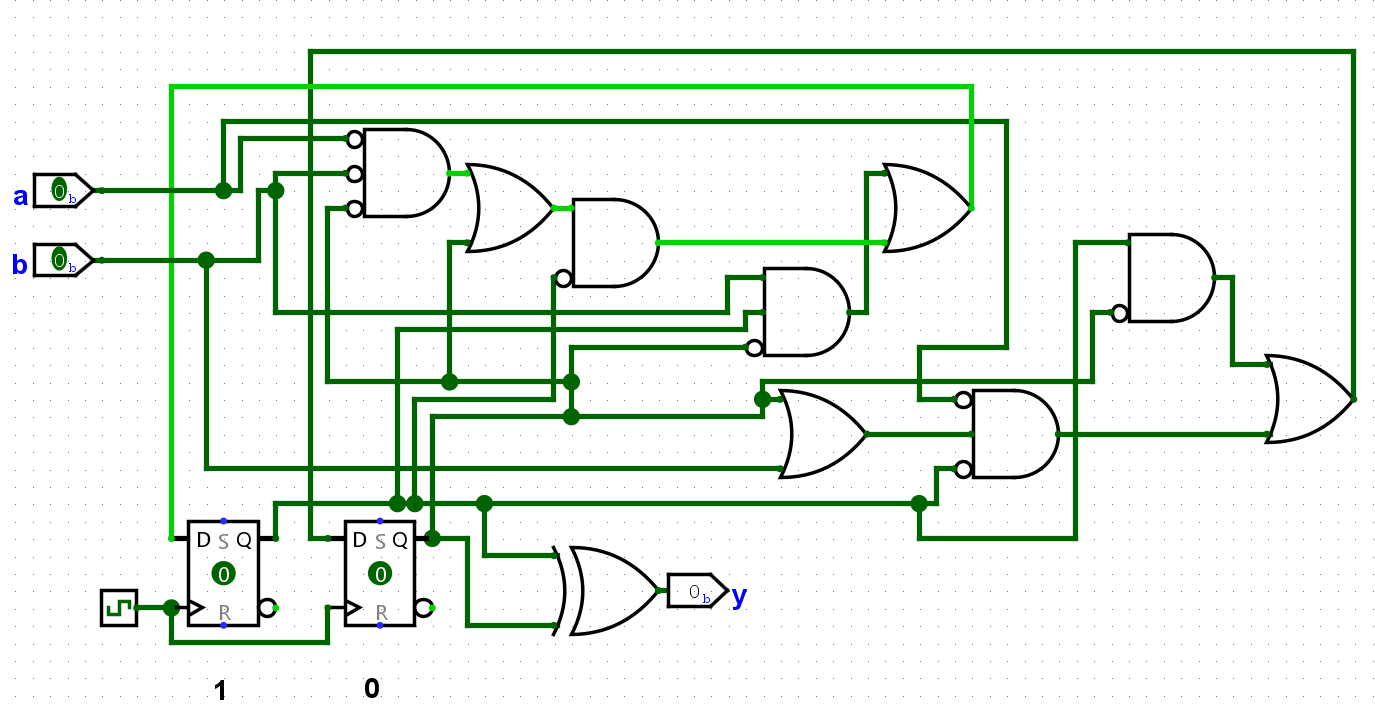
\includegraphics[width=\textwidth]{./images/3_40_circ.png}
    \caption*{Circuit implementation of the finite state machine.}
\end{figure}

\subsection*{3.43}
\begin{figure}[H]
    \centering
    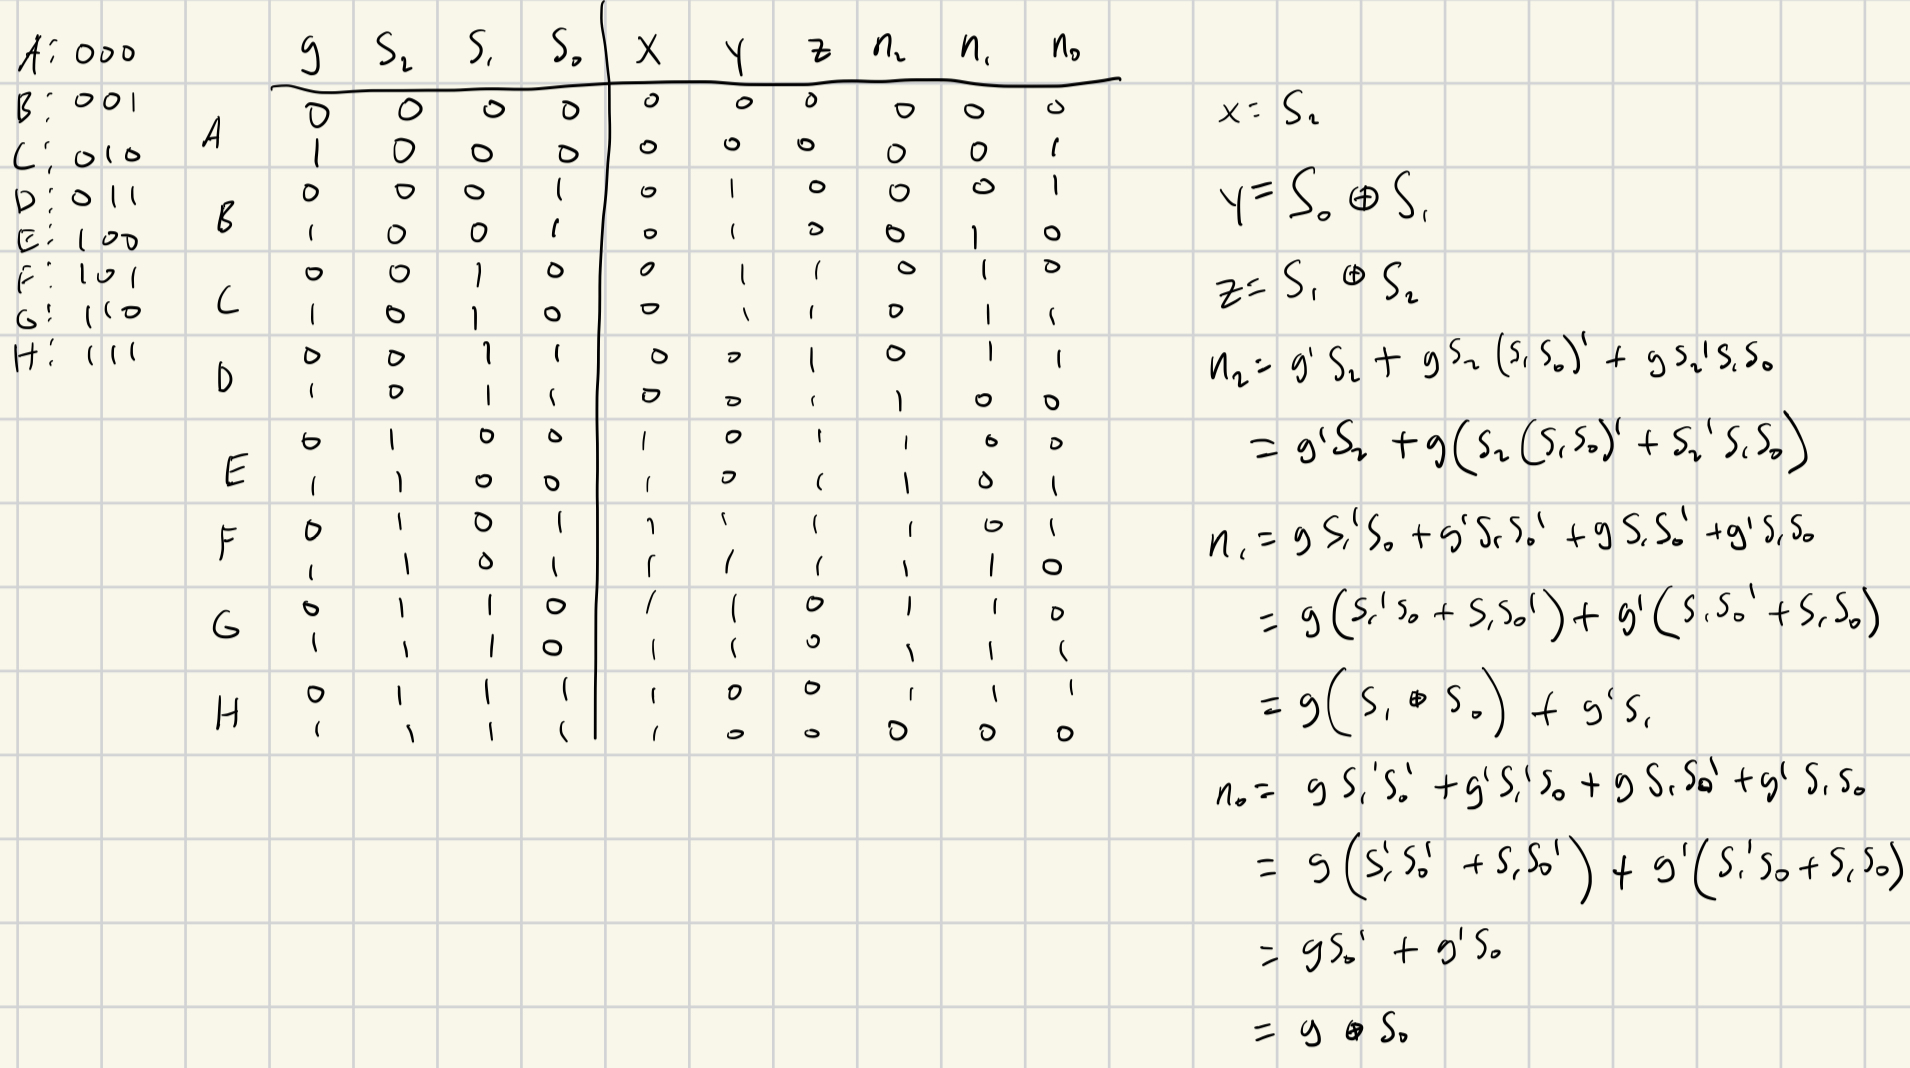
\includegraphics[width=\textwidth]{./images/3_43.jpg}
    \caption*{Truth table and boolean expressions for the finite state machine.}
\end{figure}

\begin{figure}[H]
    \centering
    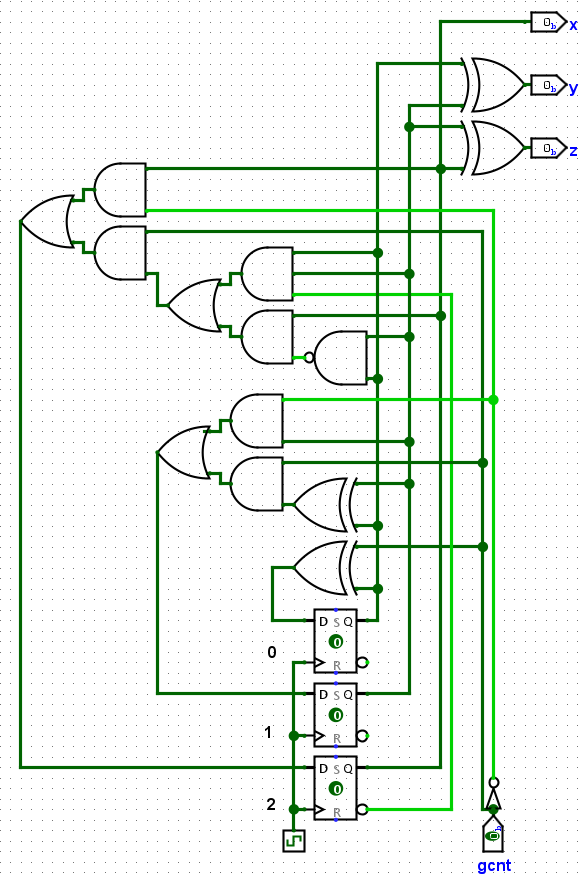
\includegraphics[width=\textwidth]{./images/3_43_circ.png}
    \caption*{Circuit implementation of the finite state machine.}
\end{figure}

\end{document}
